\documentclass[aspectratio=169,11pt]{beamer}
\usetheme{default}
\usecolortheme{default}

\setbeamertemplate{navigation symbols}{}
\setbeamertemplate{footline}[frame number]

\usepackage{amsmath}
\usepackage{booktabs}
\usepackage{graphicx}
\usepackage{tikz}
\usetikzlibrary{shapes,arrows,positioning,calc}

\newcommand{\citeslide}[1]{\hfill{\footnotesize [#1]}}

\title{Research Review: From Wave Computing to RCNs and Reaction-Diffusion}
\subtitle{Where we are, what works, and what ``computing'' could mean}
\author{Srivijayesh Venugopal}
\date{Cranfield IRP 2025-26 --- Supervisor Meeting, 15 July 2026}

\begin{document}

\begin{frame}
\titlepage
\end{frame}


% ---------------------------------------------------------------------
\begin{frame}{The journey so far}

\begin{table}
\centering
\footnotesize
\begin{tabular}{p{2.6cm}p{5.5cm}cc}
\toprule
\textbf{Direction} & \textbf{What it is} & \textbf{Spatial?} & \textbf{Works?} \\
\midrule
Acoustic porous medium & Sound waves in structured solid & Yes & Promising in principle \\
Well-mixed RCN & Trainable mass-action ODEs & No & XOR solved \\
DNA WTA & Strand-displacement neural network & No & Elegant, not aligned \\
Gray-Scott RD & Activator-inhibitor spot patterns & Yes & Patterns form \\
FitzHugh-Nagumo & Nerve-like pulses in channels & Yes & Pulses route \\
\textbf{Oregonator BZ} & \textbf{Real excitable BZ chemistry} & \textbf{Yes} & \textbf{Waves + collision} \\
\bottomrule
\end{tabular}
\end{table}

\end{frame}

% ---------------------------------------------------------------------
\begin{frame}{Phase 1: acoustic wave computing (original premise)}

Project premise: \textit{physical fluid-based neural computation}.

\vspace{0.3cm}
\begin{itemize}
    \item Continuous processing across a structured domain.
    \item Trainable geometry encodes the weights.
    \item Parallel independent inference streams.
\end{itemize}

\vspace{0.3cm}
We started with acoustic waves in a porous / structured medium:
\begin{itemize}
    \item Helmholtz / JCA acoustic modelling.
    \item Frequency-dependent transmission through obstacle arrays.
\end{itemize}

\end{frame}

% ---------------------------------------------------------------------
\begin{frame}{Phase 2: recurrent chemical network (RCN)}

Dack-style RCN \citeslide{Dack et al., 2026}: fast perceptron species $Y_j$ plus slow executive species $X_i$.
\begin{align*}
    \frac{dX_i}{dt} &= \beta_i + X_i \sum_j \alpha_{ij} Y_j \\
    \mu \frac{dY_j}{dt} &= \gamma + \theta_j Y_j + Y_j \sum_i \omega_{ji} X_i - Y_j^2
\end{align*}

\vspace{0.2cm}
\begin{itemize}
    \item $Y_j$ act as a smooth ReLU-like layer.
    \item $X_i$ hold inputs and output.
    \item Trained with L-BFGS-B; recurrent version solves XOR.
\end{itemize}

\vspace{0.2cm}
\centering
\textbf{Result:} a trainable chemical ODE can learn a non-linear function.

\end{frame}

% ---------------------------------------------------------------------
\begin{frame}{RCN result: XOR}

\centering
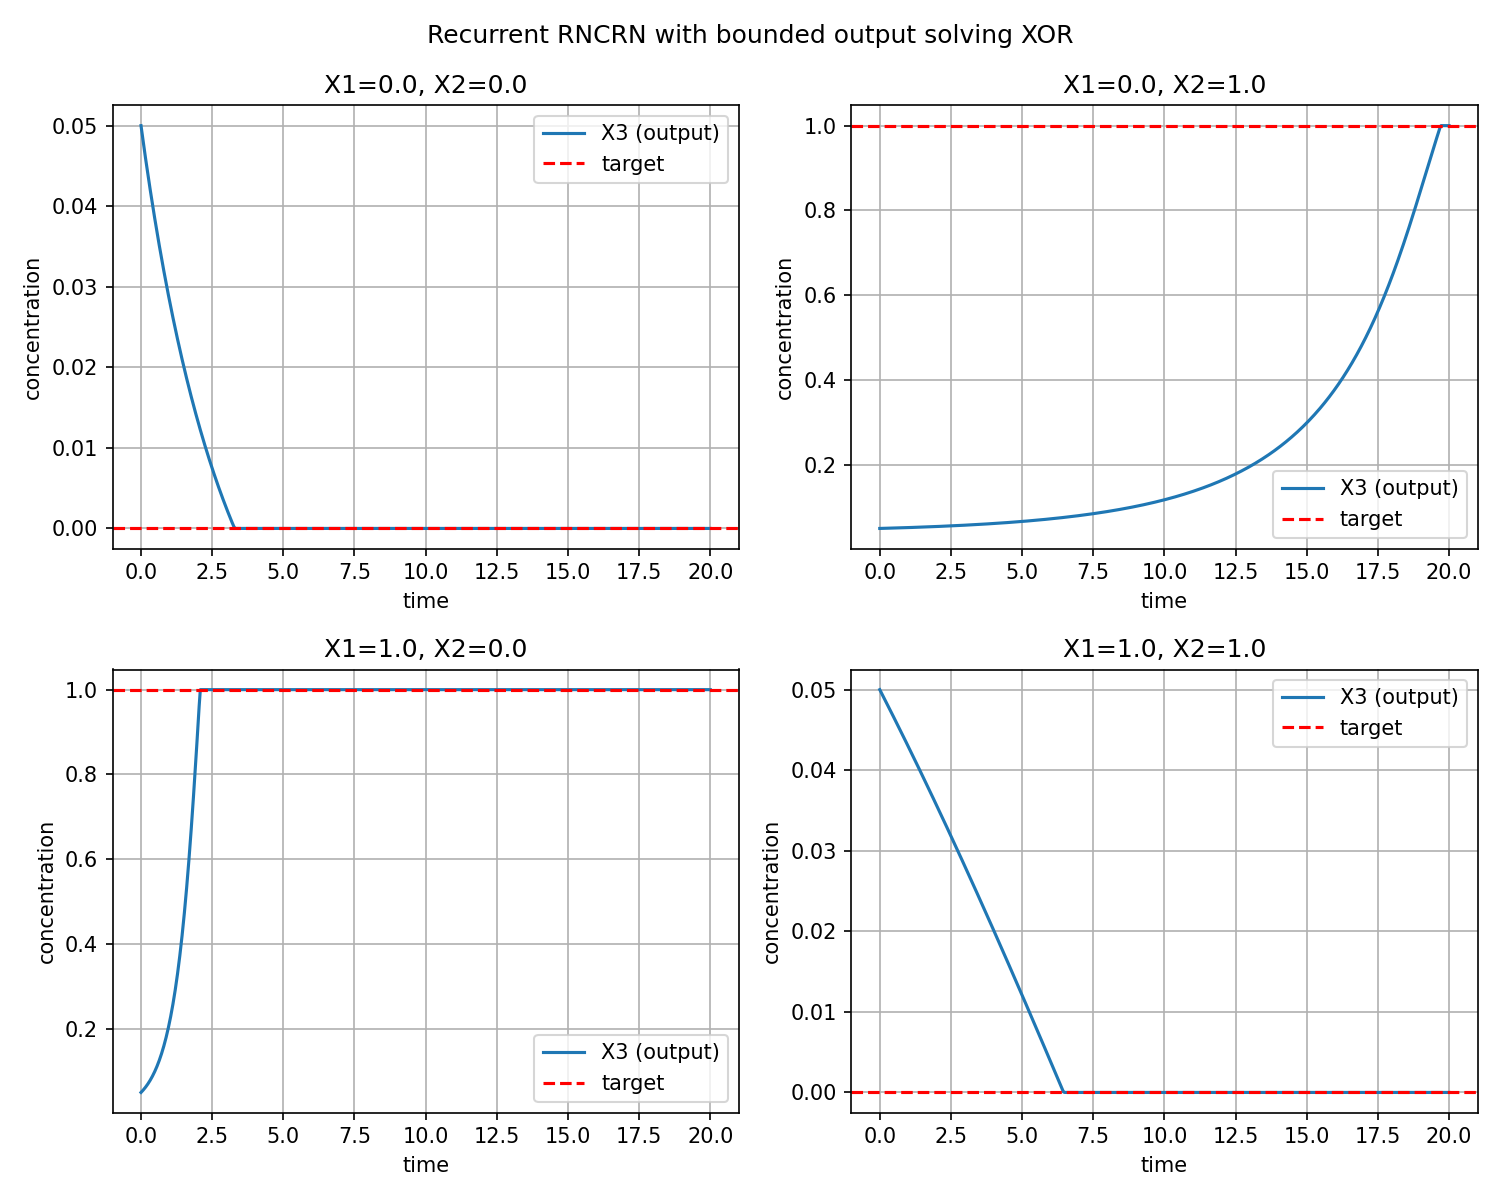
\includegraphics[width=0.55\textwidth]{../Analysis/dack_rncrn_xor_recurrent_bounded_results.png}

\vspace{0.2cm}
Limitation: well-mixed, no spatial continuity, trainable parameters are rate constants. Reactions are arbitrary; need mapping and control to real world reactions.

\end{frame}

% ---------------------------------------------------------------------
\begin{frame}{Phase 3: DNA winner-take-all}

Cherry \& Qian 2018 \citeslide{Cherry \& Qian, Nature 2018}: DNA WTA neural network.

\vspace{0.2cm}
\begin{itemize}
    \item Weights = DNA strand concentrations.
    \item Classifies 100-bit MNIST patterns into 9 digits.
    \item Works well, but \textbf{well-mixed} and requires specialist sequence design.
\end{itemize}

\vspace{0.3cm}
\textbf{Limitations:}
\begin{itemize}
    \item Not spatially continuous.
    \item Trainable parameters are molecular concentrations, not geometry or flow.
    \item Weak link to the ``parallel independent inference streams'' idea.
\end{itemize}

\vspace{0.2cm}
\centering
This pushed us toward \textbf{spatial reaction-diffusion}.

\end{frame}

% ---------------------------------------------------------------------
\begin{frame}{Phase 4: reaction-diffusion computing}

Three candidate models tested:

\vspace{0.3cm}
\begin{table}
\centering
\footnotesize
\begin{tabular}{p{2.8cm}p{5.5cm}c}
\toprule
\textbf{Model} & \textbf{What it does} & \textbf{Real chemistry?} \\
\midrule
Gray-Scott & Spots / stripes from activator-inhibitor kinetics & No \\
FitzHugh-Nagumo & Nerve-like pulse propagation & No \\
Barkley & Reduced BZ excitable medium & Phenomenological \\
Oregonator & BZ chemistry with HBrO$_2$ + catalyst & Yes \\
\bottomrule
\end{tabular}
\end{table}

\vspace{0.3cm}
\centering
All four are spatial, continuous media. The question is which one can be \textit{trained}.

\end{frame}

% ---------------------------------------------------------------------
\begin{frame}{Gray-Scott: pattern formation}

Gray-Scott equations:
\begin{align*}
    \frac{\partial U}{\partial t} &= D_U \nabla^2 U - UV^2 + F(1-U) \\
    \frac{\partial V}{\partial t} &= D_V \nabla^2 V + UV^2 - (F+k)V
\end{align*}

\vspace{0.2cm}
\begin{itemize}
    \item $U$ = activator feed, $V$ = inhibitor, $F$ and $k$ control morphology.
    \item A central seed of $V$ evolves into stable spot patterns.
\end{itemize}

\vspace{0.2cm}
\footnotesize
This proves the medium supports robust, self-organised spatial structures.

\end{frame}

% ---------------------------------------------------------------------
\begin{frame}{Barkley: BZ phenomenology}

Barkley reduction of BZ:
\begin{align*}
    \frac{\partial u}{\partial t} &= D_u \nabla^2 u + \frac{1}{\varepsilon} u(1-u)\left(u - \frac{v+b}{a}\right) \\
    \frac{\partial v}{\partial t} &= D_v \nabla^2 v + u - v
\end{align*}

\vspace{0.2cm}
\centering
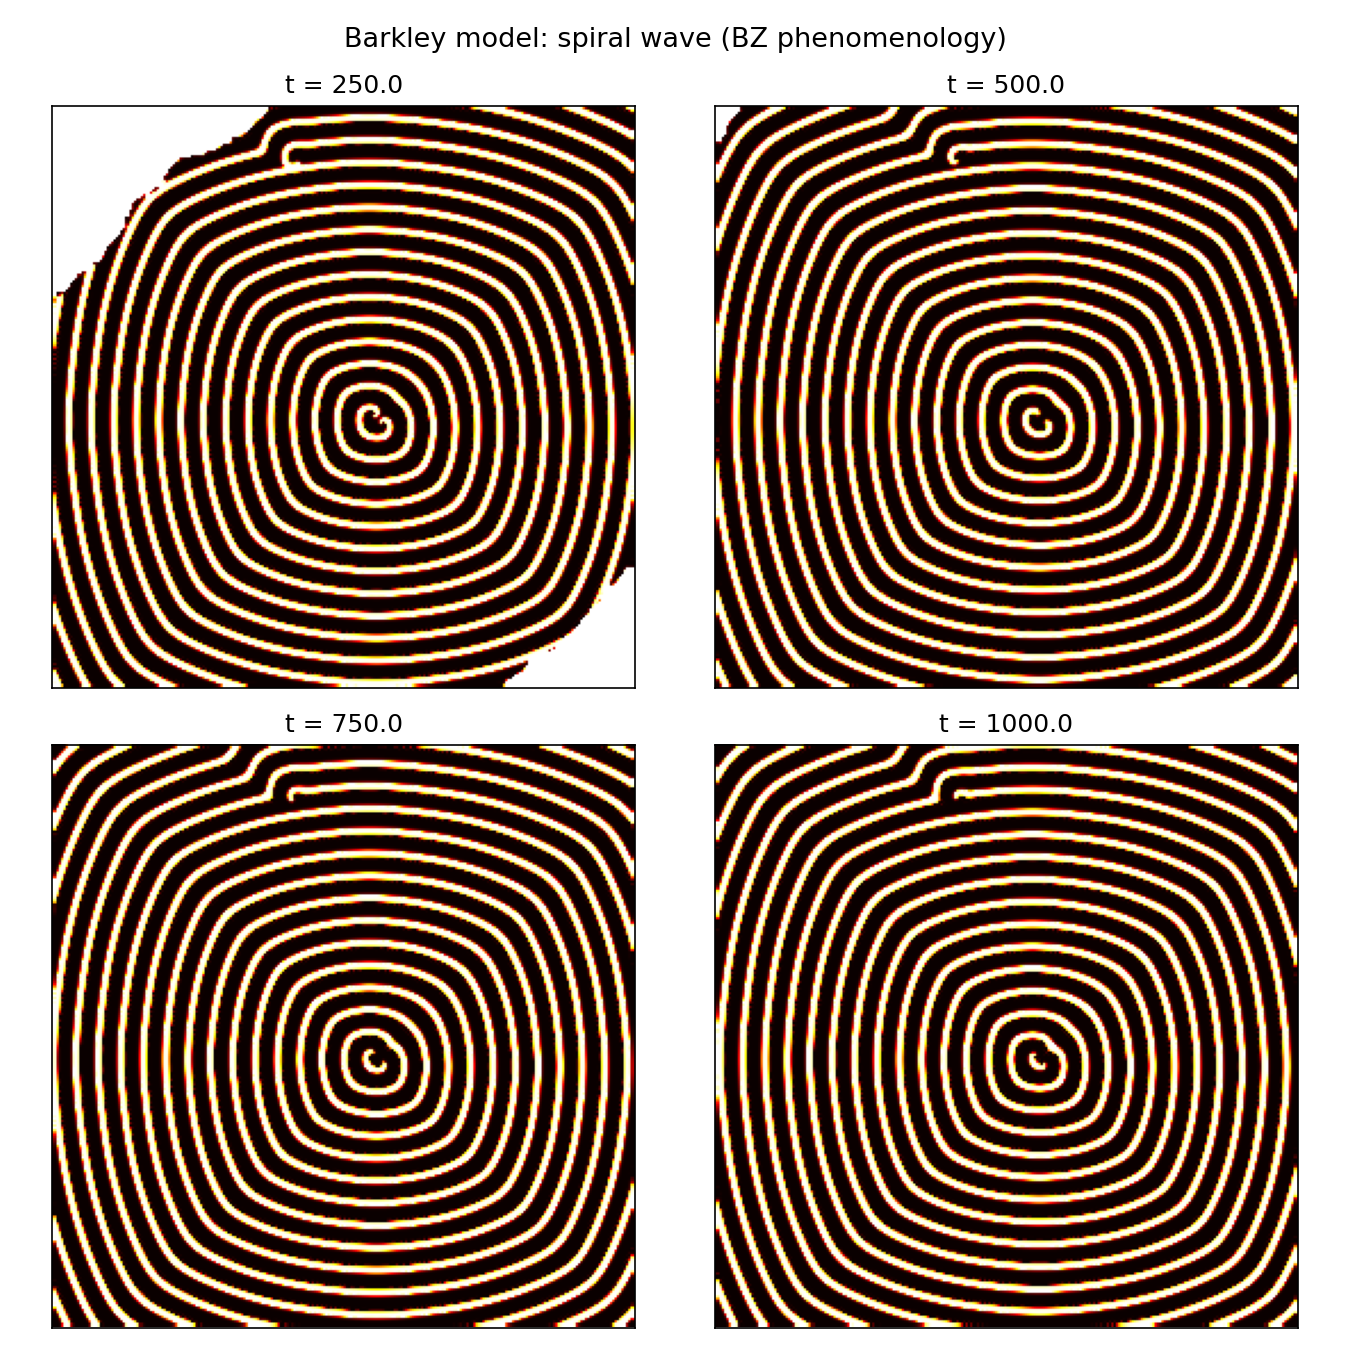
\includegraphics[width=0.35\textwidth]{../Analysis/barkley_spiral.png}

\end{frame}

% ---------------------------------------------------------------------
\begin{frame}{Oregonator: chemically grounded BZ waves}

Oregonator equations:
\begin{align*}
    \frac{\partial u}{\partial t} &= D_u \nabla^2 u + \frac{1}{\varepsilon}\left[ u - u^2 - (f v + \phi)\frac{u-q}{u+q} \right] \\
    \frac{\partial v}{\partial t} &= D_v \nabla^2 v + u - v
\end{align*}

\vspace{0.2cm}
\begin{itemize}
    \item $u \sim$ HBrO$_2$, $v \sim$ oxidised catalyst Ce(IV).
    \item $\phi(x,y)$ = light-induced suppression, a spatially tunable field.
    \item Robust target waves, collision, and diffraction.
\end{itemize}

\vspace{0.2cm}
\centering
\textbf{This is our current best forward solver.}

\end{frame}

% ---------------------------------------------------------------------
\begin{frame}{Oregonator result 1: target waves}

\centering
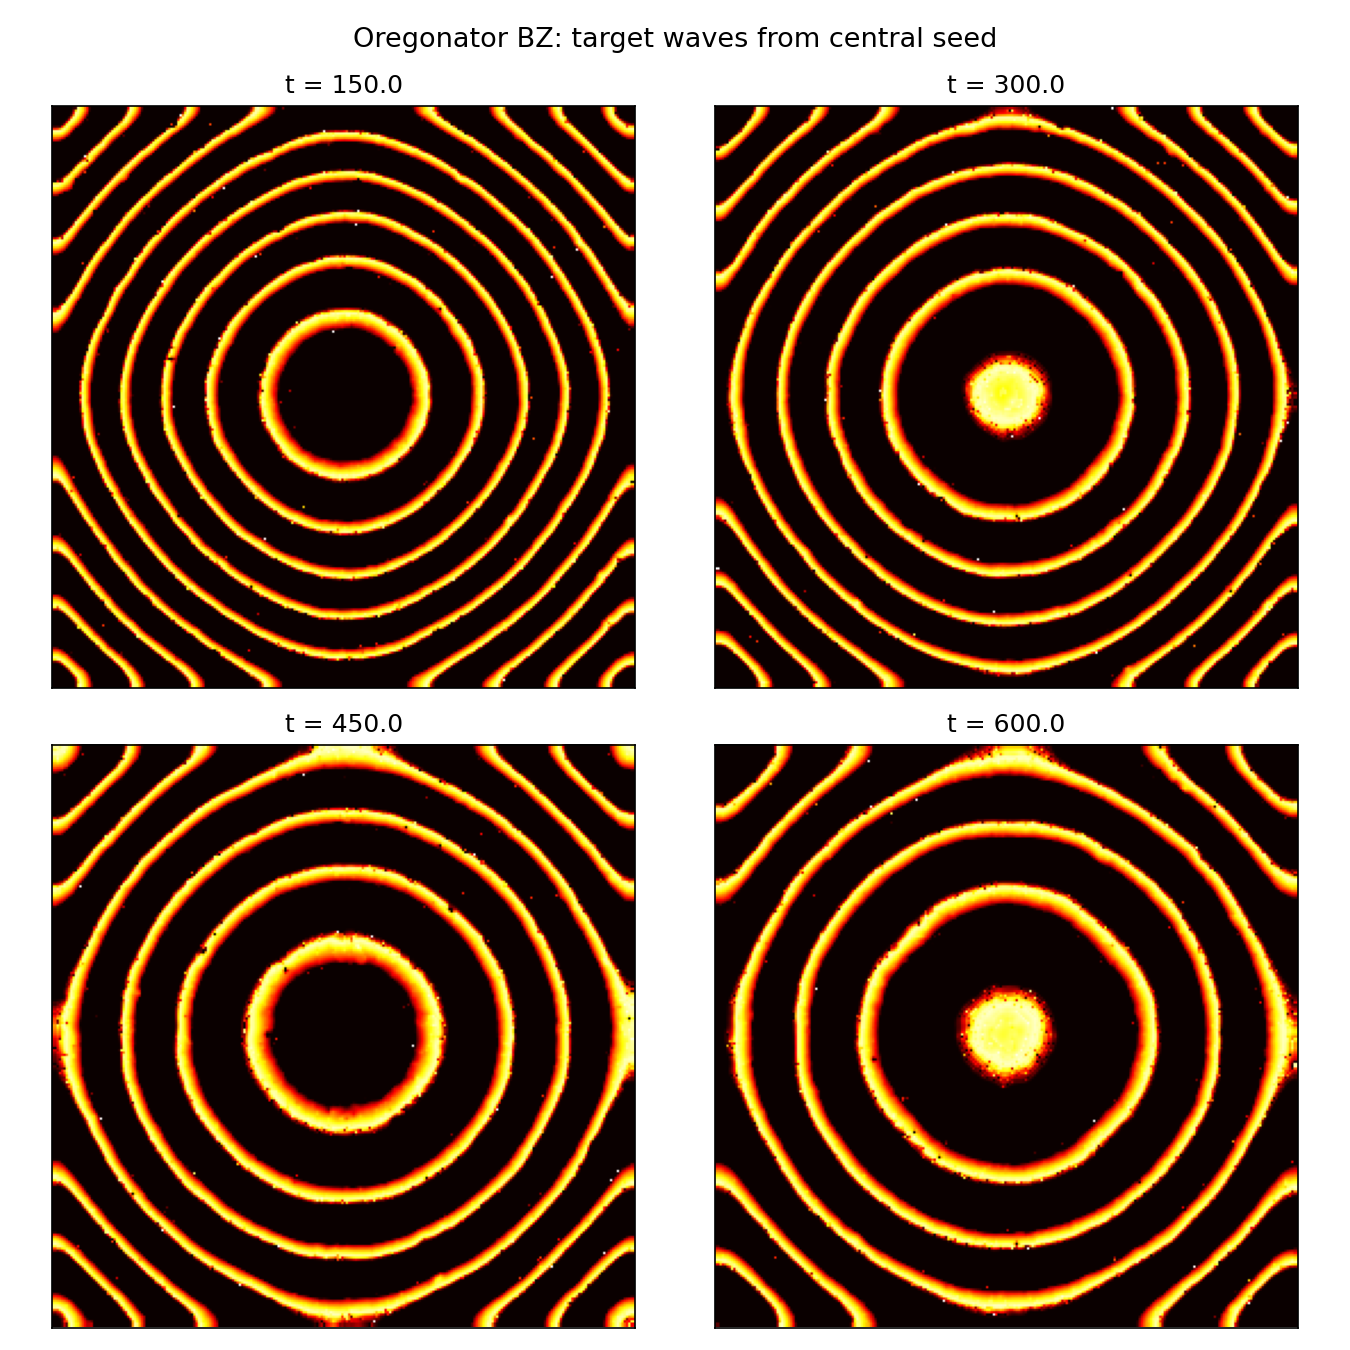
\includegraphics[width=0.60\textwidth]{../Analysis/oregonator_target.png}

\vspace{0.3cm}
A small excited seed emits circular target waves --- the basic propagating signal.

\end{frame}

% ---------------------------------------------------------------------
\begin{frame}{Oregonator result 2: counter-propagating waves}

\centering
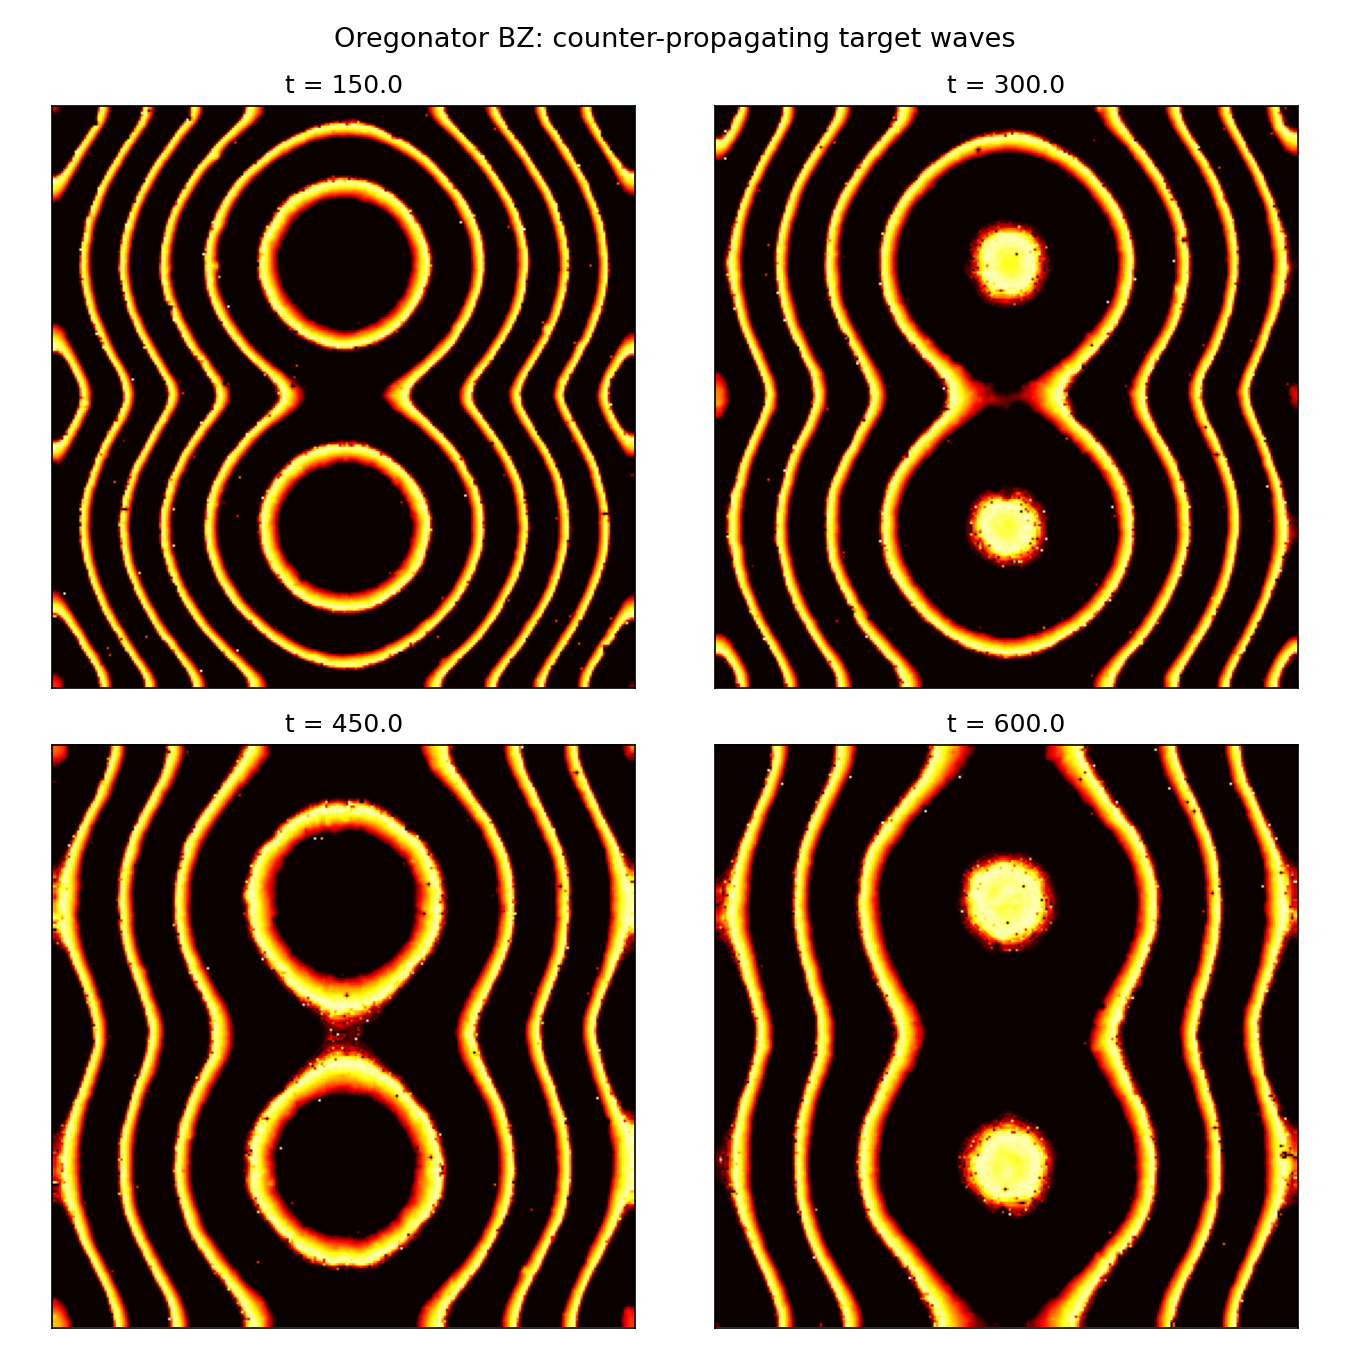
\includegraphics[width=0.60\textwidth]{../Analysis/oregonator_collision.png}

\vspace{0.3cm}
Two target waves meet and suppress each other in the overlap region.

\end{frame}

% ---------------------------------------------------------------------
\begin{frame}{Oregonator result 3: diffraction through a gap}

\centering
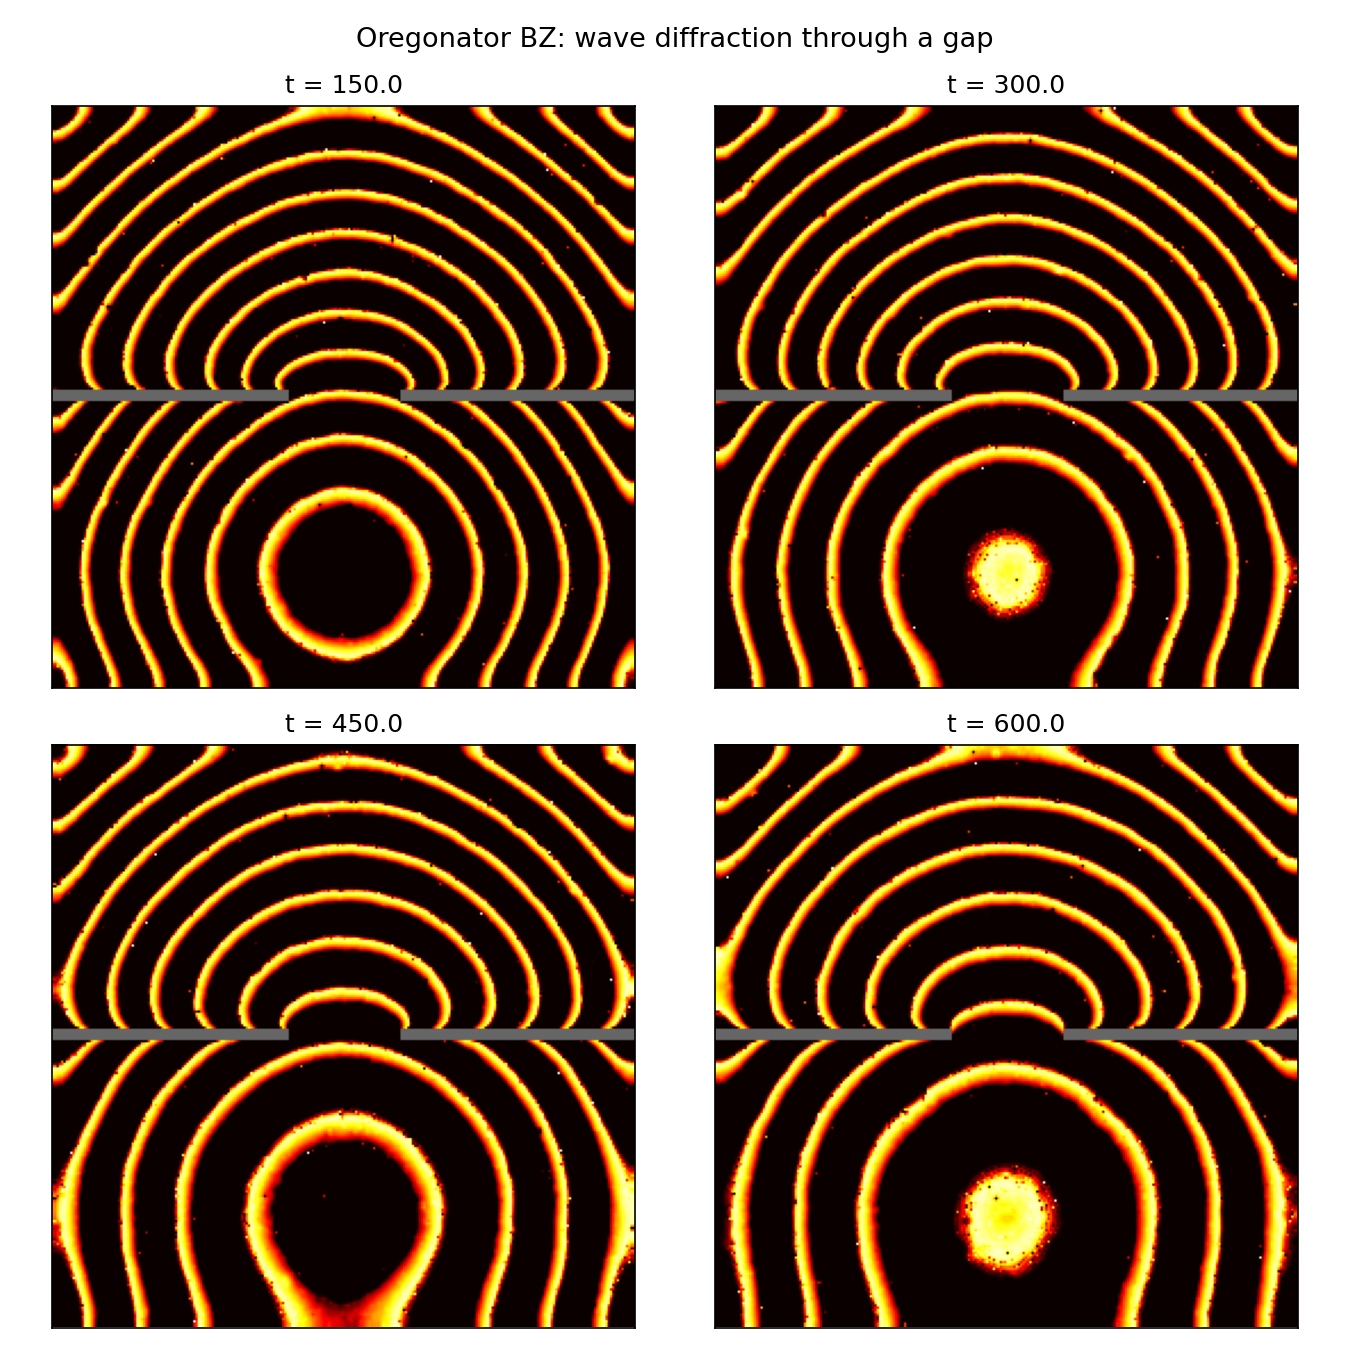
\includegraphics[width=0.60\textwidth]{../Analysis/oregonator_gap_diffraction.png}

\vspace{0.3cm}
A no-flux wall with a gap blocks most of the wave; the fragment diffracts through.

\end{frame}

% ---------------------------------------------------------------------
\begin{frame}{Oregonator result 4: timing as a control parameter}

\centering
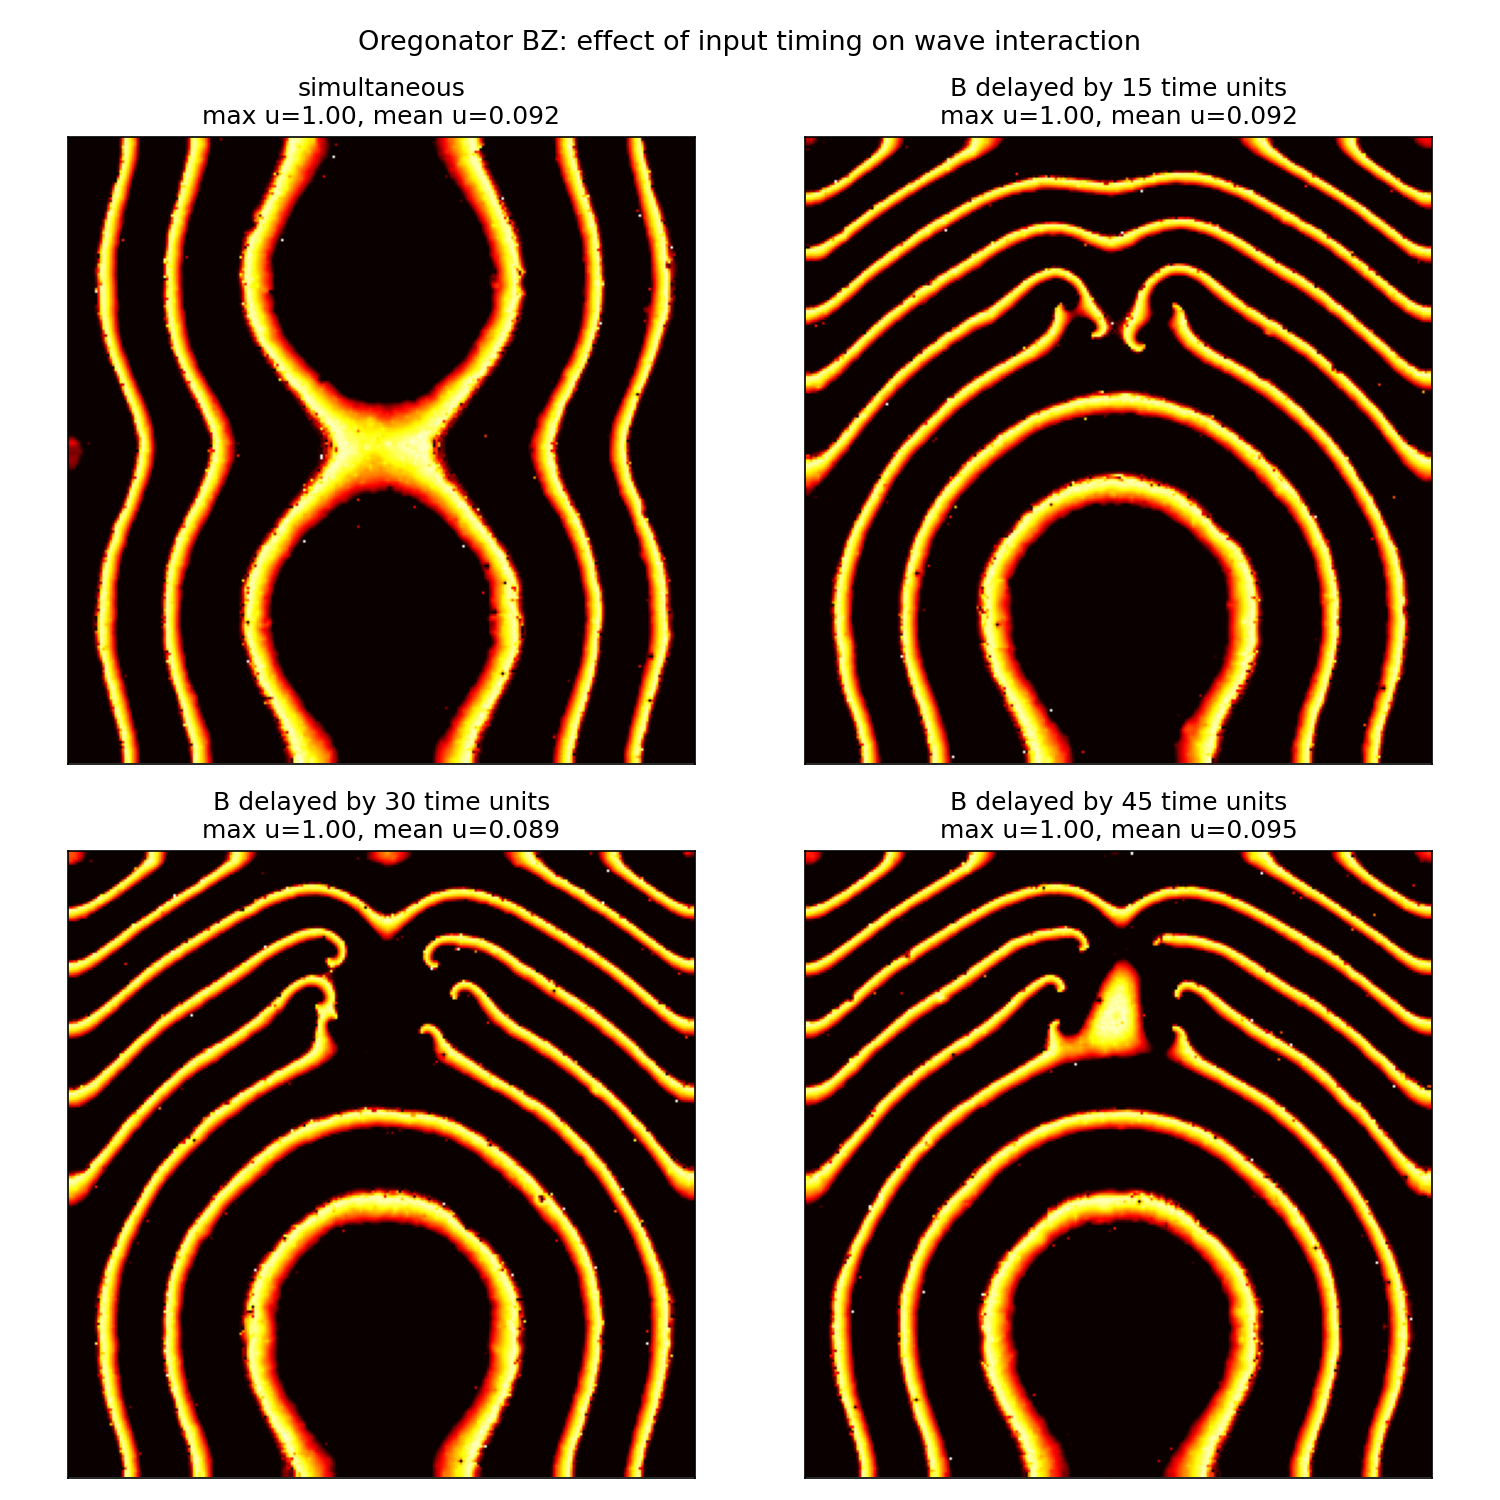
\includegraphics[width=0.55\textwidth]{../Analysis/oregonator_timing_sweep.png}

\vspace{0.3cm}
\footnotesize
Two excitation pulses are initiated at different delays. The arrival time at the readout probe changes with the offset, giving a third trainable layer alongside geometry and the excitability field.

\end{frame}

% ---------------------------------------------------------------------
\begin{frame}{The central question: can pattern formation compute?}

We now have spatial, continuous dynamics. But how do we turn them into a computer?

\vspace{0.3cm}
Three paradigms from the literature:

\vspace{0.2cm}
\begin{enumerate}
    \item \textbf{Wave-collision logic} \citeslide{Adamatzky \& De Lacy Costello, 2002}
    \begin{itemize}
        \item Pulses annihilate or merge at junctions \textrightarrow{} AND, OR, XOR.
    \end{itemize}
    \item \textbf{Pattern-as-state}
    \begin{itemize}
        \item Final spatial pattern encodes the answer; read out at fixed probes.
    \end{itemize}
    \item \textbf{Trainable field}
    \begin{itemize}
        \item Optimise geometry or excitability map so inputs evolve to target outputs.
    \end{itemize}
\end{enumerate}

\vspace{0.3cm}
\centering
Which paradigm is the right one for this thesis?

\end{frame}

% ---------------------------------------------------------------------
\begin{frame}{Paradigm 1: wave-collision logic}

Pros:
\begin{itemize}
    \item Directly maps to Boolean gates (OR, AND, XOR).
    \item Experimentally demonstrated in BZ.
    \item Natural fit to channel geometry.
\end{itemize}

Cons:
\begin{itemize}
    \item Timing matters: simultaneous pulses annihilate, offset ones may not.
    \item Hard to scale beyond small circuits.
    \item Each gate is a one-shot pulse, not a reusable neuron.
\end{itemize}

\vspace{0.3cm}
\centering
Best for: a small demo of ``chemical logic'', not a trainable architecture.

\end{frame}

% ---------------------------------------------------------------------
\begin{frame}{Paradigm 2: pattern-as-state}

Pros:
\begin{itemize}
    \item Gray-Scott already makes rich stable patterns.
    \item Input can be an initial condition; output is a final pattern.
    \item Readout at probe locations is simple.
\end{itemize}

Cons:
\begin{itemize}
    \item Pattern-to-function mapping is not obvious.
    \item Small input changes may cause large, unpredictable pattern changes.
    \item Less connected to the ``wave routing'' intuition.
\end{itemize}

\vspace{0.3cm}
\centering
Best for: classification via evolved patterns, if we can train the morphology map.

\end{frame}

% ---------------------------------------------------------------------
\begin{frame}{Paradigm 3: trainable field / geometry}

Pros:
\begin{itemize}
    \item Matches Project 11: trainable architecture.
    \item Light field $\phi(x,y)$ in Oregonator is a natural continuous control.
    \item Channel walls give discrete topology optimisation.
\end{itemize}

Cons:
\begin{itemize}
    \item Forward solve must be robust (Oregonator is).
    \item Optimisation landscape may be rough.
    \item Need to define input encoding, readout, and loss carefully.
\end{itemize}

\vspace{0.3cm}
\centering
Best for: a trainable continuous computing medium.

\end{frame}

% ---------------------------------------------------------------------
\begin{frame}{What I think the answer looks like}

A hybrid: \textbf{designed geometry guides the waves; trainable parameters tune the response}.

\vspace{0.3cm}
\begin{center}
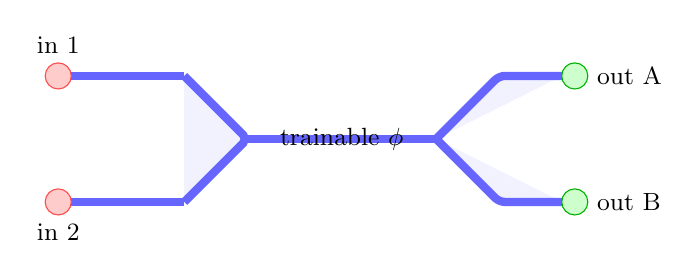
\begin{tikzpicture}[scale=0.8,
    channel/.style={draw=blue!60, line width=3pt, rounded corners=2pt, fill=blue!5},
    input/.style={draw=red!70, fill=red!20, circle, minimum size=6pt},
    output/.style={draw=green!70!black, fill=green!20, circle, minimum size=6pt}]

\draw[channel] (0,2) -- (2,2);
\draw[channel] (0,0) -- (2,0);
\draw[channel] (2,2) -- (3,1) -- (2,0);
\draw[channel] (3,1) -- (6,1);
\draw[channel] (6,1) -- (7,2) -- (8,2);
\draw[channel] (6,1) -- (7,0) -- (8,0);

\node[input] at (0,2) {};
\node[input] at (0,0) {};
\node[output] at (8.2,2) {};
\node[output] at (8.2,0) {};
\node[right] at (8.4,2) {\small out A};
\node[right] at (8.4,0) {\small out B};
\node[above] at (0,2.2) {\small in 1};
\node[below] at (0,-0.2) {\small in 2};
\node at (4.5,1) {\small trainable $\phi$};
\end{tikzpicture}
\end{center}

\vspace{0.3cm}
\begin{itemize}
    \item Inputs: excitation pulses at ports.
    \item Medium: Oregonator BZ in a channel network.
    \item Trainable: wall positions and/or light-suppression field.
    \item Output: read $u$ at probe locations after a fixed time.
\end{itemize}

\end{frame}

% ---------------------------------------------------------------------
\begin{frame}{Proposed next steps}

\begin{enumerate}
    \item \textbf{Implement the optimisation loop} around the Oregonator forward solve.
    \item \textbf{First task:} 2-to-1 pulse router (OR gate) in a channel.
    \item \textbf{Second task:} XOR by training geometry/field so two inputs annihilate.
    \item \textbf{Compare:} trainable field vs.~trainable geometry.
    \item \textbf{Write up:} physics, numerical method, and limitations.
\end{enumerate}

\vspace{0.3cm}
\centering
\textbf{If this works, we have a continuous, spatial, trainable computing primitive for Project 11.}

\end{frame}

% ---------------------------------------------------------------------
\begin{frame}{What I need from you}

\begin{enumerate}
    \item \textbf{Validate the direction:} Is Oregonator BZ + trainable geometry the right thesis core?
    \item \textbf{Pick the computing paradigm:} Wave logic, pattern-as-state, or trainable field?
    \item \textbf{Scope check:} Should we aim for one trained gate, or a small circuit?
    \item \textbf{Methodology:} Is gradient-free optimisation acceptable, or should we pursue adjoint/gradient methods?
\end{enumerate}

\end{frame}

% ---------------------------------------------------------------------
\begin{frame}{References}

{\footnotesize
\begin{enumerate}
    \item A. Dack \textit{et al.} Recurrent neural chemical reaction networks that approximate arbitrary dynamics. \textit{Cell Systems}, 2026.
    \item K. M. Cherry \& L. Qian. Scaling up molecular pattern recognition with DNA-based winner-take-all neural networks. \textit{Nature} 559, 370--376 (2018).
    \item A. Adamatzky \& B. De Lacy Costello. Experimental logical gates in a reaction-diffusion medium. \textit{Phys. Rev. E} 66, 046112 (2002).
    \item J. J. Tyson \& P. C. Fife. Singular perturbation analysis of the Oregonator model. \textit{J. Chem. Phys.} 73, 2224 (1980).
    \item T. T\'oth \& K. Showalter. Logic gates in excitable media. \textit{J. Chem. Phys.} 103, 2058 (1995).
\end{enumerate}
}

\end{frame}

\end{document}
